%!TEX root = ../../../thesis.tex

\chapter{Automating Build and Deployment with CI/CD}
\label{ch:p1:cicd}

\dictum[Edsger W. Dijkstra]{%
  If debugging is the process of removing software bugs, then programming must be the process of putting them in. }%
\vskip 1em

\readit{1}

\tldr{CICD intro, git private}
This chapter describes the continuous integration testing and deployment (CI/CD) pipeline as introduced in \openqxd's development repository\cite{gitlab:openqxd-devel}.
At the time of writing this thesis the repository is private.
As part of the goals of the PASC project\cite{pasc:project} and thus as part of this thesis, we instantiated CI/CD paradigms to the development workflow of \openqxd.
This chapter details our strategy for continuous integration (\cref{sec:cicd:integration}), continuous testing directly on target hardware at CSCS (\cref{sec:cicd:testing}), software deployment to CSCS infrastructure (\cref{sec:cicd:deployment}) and finishes with a summary (\cref{sec:cicd:summary}).

\section{Continuous integration}
\label{sec:cicd:integration}

\tldr{CI strat, everything via merge-reqs, review, test}
New features, bug-fixes or code changes enter the codebase by means of a separate branch and a corresponding merge-request, which is reviewed, tested and finally merged to the master branch.
The master branch stays clean and functional, such that at every point in time one can release a new version of the software by just taking the newest commit to the master branch as version tag.

\section{Continuous testing}
\label{sec:cicd:testing}

\tldr{testing gitlab+CSCS cronjob + on every merge-req}
We decided on a testing strategy as follows:
\begin{itemize}
    \item For continuous testing, the master branch is tested on a daily basis overnight at 1 am (CET) on local resources at ETH. This runs the GitLab pipeline described in \cref{sec:cicd:pipeline:gitlab}.
    \item For continuous testing, the master branch is tested every 3 months on GH200 machines at CSCS. This runs the CSCS pipeline described in \cref{sec:cicd:pipeline:cscs}.
    \item For continuous integration, every commit into every open merge-request is automatically tested on local resources at ETH. This runs the GitLab pipeline described in \cref{sec:cicd:pipeline:gitlab}.
    \item{For continuous integration, open merge-requests can be tested by triggering the CSCS pipeline manually. This runs the CSCS pipeline described in \cref{sec:cicd:pipeline:cscs}. The pipeline can be trigger by commenting on any merge-request with \code{cscs-ci run default}, see \cref{fig:cicd:comment}. This will invoke a webhook that triggers CSCS services to pull the repository and run the pipeline. A short time after commenting, a new job appears in the pipeline view with stage external, see \cref{fig:cicd:external}.}
\end{itemize}

\begin{figure}
    \centering
    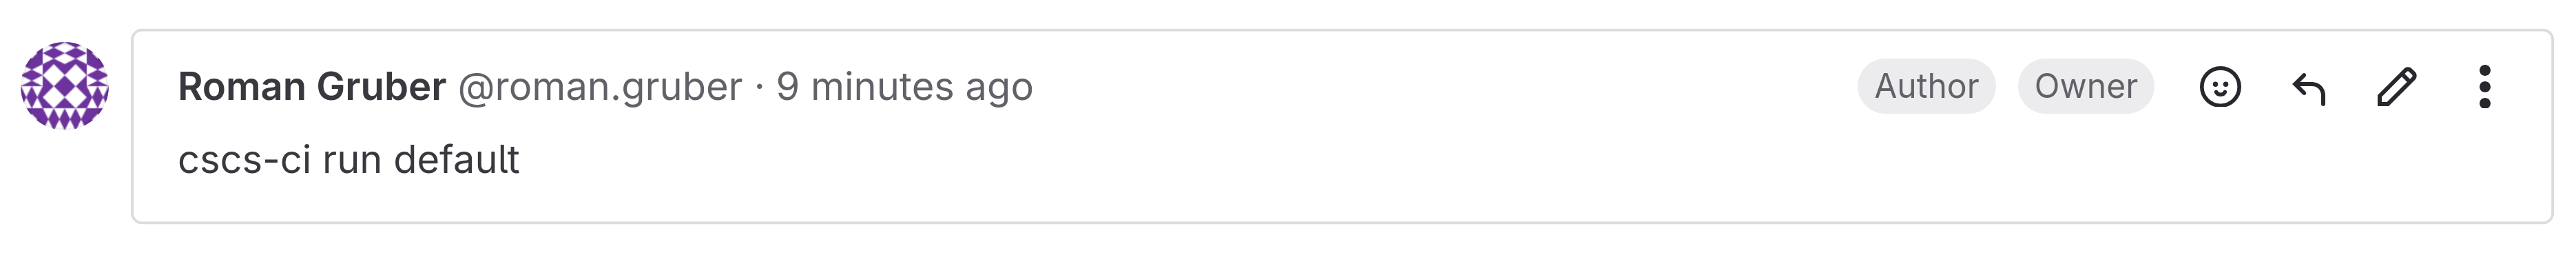
\includegraphics[width=\linewidth]{\dir/img/comment.png}
    \caption{The comment to add to a pull-request that starts the CSCS default pipeline.}
    \label{fig:cicd:comment}
\end{figure}

\begin{figure}
    \centering
    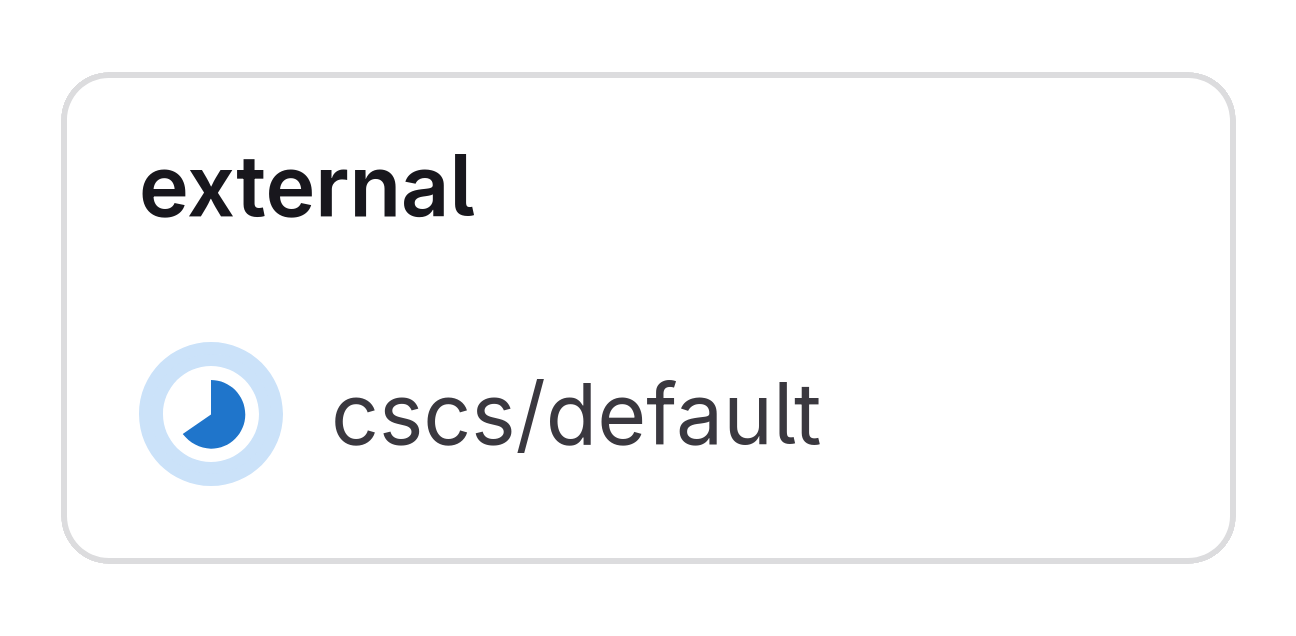
\includegraphics[width=100px]{\dir/img/default.png}
    \caption{The job in the external stage that represents the CSCS default pipeline. One can click on the job to be redirected to CSCS servers where the whole pipeline including status of the jobs is visible.}
    \label{fig:cicd:external}
\end{figure}

\tldr{2 pipelines: gitlab + CSCS}
Thus there are two separate pipelines.
One that runs on via GitLab on local resources at ETH, and one that runs via CSCS on GH200 nodes at CSCS.
Both pipelines are independent and completely detached from each other, they may run in parallel or not.

\subsection{GitLab pipeline}
\label{sec:cicd:pipeline:gitlab}

\tldr{ETH runner, GPU required but not for all jobs}
The entrypoint for the local GitLab pipeline is in the openQxD-devel repository\cite{gitlab:openqxd-devel} under \code{.gitlab-ci.yml} directly in the root.
Parts of this pipeline may run on official GitLab runners (if time is available).
The test jobs require runners to expose one or more local NVIDIA GPUs to the docker image to be able to run CUDA code.
Clearly the official GitLab runners do not provide GPUs.
We registered a local machine at ETH which specifications
\begin{itemize}
    \item 2x AMD EPYC 9124 16-Core Processor
    \item 8x NVIDIA GeForce A2000 (12 GB, CUDA-architecture \code{sm\_86})
    \item 1.5 TB main memory
\end{itemize}
as an additional runner for this pipeline. The machine has 8 GPUs which makes it ideal for various testing scenarios, like lattices with C$^\star$-boundaries in all $3$ spatial directions which require a minimum of 8 ranks.

\tldr{Split into stages}
The pipeline consists of three stages; prepare, build and test.
In general the stages depends on each other, although there are jobs in the build stage which depend on nothing.
The individual stages will be discussed separately in the following.

\subsubsection{The prepare stage}

\tldr{prep stage, can run everywhere, artifacts, qudas develop branch}
\emph{All jobs in the prepare stage may run on official GitLab runners.}
As the name suggests, this stage has some preparatory jobs, whose artifacts will be exposed to subsequent jobs.
The job called \code{download-quda} downloads a copy of \quda from its official GitHub repository \cite{github:quda} via \code{git clone} and exposes it as artifact.
We download the latest developments committed to the \code{develop} branch, \ie their CI branch.
All subsequent tests that depend on this job, will use the newest available developments of \quda.
Therefore, we will notice breaking changes immediately.

\subsubsection{The build stage}
\label{sec:cicd:pipeline:gitlab:build}

\tldr{build, runs everywhere, matrix of MPI+CC, job name pattern}
\emph{All jobs in the build stage may run on official GitLab runners.}
However, this stage consists of a matrix of jobs that compile \openqxd with various combinations of compilers and MPI implementations.
This can be easily extended to cover missing combinations.
At the time of writing, we cover compilers gcc-10, gcc-11, gcc-12, gcc-13, gcc-14, clang-18 and two MPI libraries \openmpi~\cite{online:openmpi} and MPICH~\cite{online:mpich}.
These compile-jobs search through the whole repository.
In every directory they find a \code{Makefile}, they will call \code{make}.
This makes sure that all programs and modules in the project are compiled.
These jobs do not depend on any other job and will fail if one of the \code{make} commands fails.
Their job names have the pattern
\begin{minted}[linenos=false]{text}
build-openqxd/<mpi>:<version>-<compiler>:<version>
\end{minted}
where \code{<mpi>} is replaced by either \code{openmpi} or \code{mpich} and \code{<compiler>} with \code{gcc} or \code{clang} and their respective versions.

\tldr{depend on prep/build, build quda jobs}
The remaining build jobs may depend on the prepare stage or on other build jobs.
The jobs with pattern
\begin{minted}[linenos=false]{text}
build-quda/cuda:<version>-<cuda_arch>
\end{minted}
build \quda for the CUDA architecture given by \code{<cuda\_arch>} using certain CUDA versions given by \code{<version>}. 
They can also easily be extended to cover more versions and architectures.

\tldr{build openqxd vs quda, their deps, BCs, lattices}
Finally the jobs to build \openqxd against \quda have the pattern
\begin{minted}[linenos=false]{text}
build-openqxd/quda-checks/<cuda_arch>-<bcs>
\end{minted}
They depend on the previous build jobs that build \quda with the corresponding \code{<cuda\_arch>}.
The placeholder \code{<bcs>} is substituted with the boundary conditions of the lattice we want to test against.
Currently we run tests on two lattices, see \cref{tab:cicd:ensembles}.
Thus we compile \openqxd on a process grid of 1x2x2x2 with 8 ranks for these two lattices.
Again this can be extended to other lattices.

\begin{table}[t]
  \centering
  \begin{tabular}{ccccc}
    \toprule
    {ensemble}&
    {$L_0 \times L^3$}&
    {$m_{\pi}$ [MeV]}&
    {boundary conditions}&
    {\# configs} \\
    \midrule
    D5d  & $48 \times 24^3$ & 439 & periodic    & 2 \\
    A360 & $64 \times 32^3$ & 360 & C$^{\star}$ in xyz directions & 2 \\
    \bottomrule
  \end{tabular}
  \caption{\label{tab:cicd:ensembles}%
    Ensembles used in the CI/CD pipeline. The periodic lattice D5d is taken from ref.~\cite{online:cls}, whereas the C$^{\star}$ lattice is taken from ref.~\cite{RCstar22}.}
\end{table}

\subsubsection{The test stage}
\label{sec:cicd:pipeline:gitlab:test}

\tldr{deps, name pattern of test jobs, test binaries discussion}
\emph{All jobs in the test stage may \textbf{not} run on official GitLab runners, they require a GPU and thus may only run on the local resource specified above or on a registered runner exposing a GPU.}
Jobs in this stage depend on the build jobs that build \openqxd against \quda discussed at the end of the previous section.
They may not run if previous jobs in the dependency chain failed.
They have names as
\begin{minted}[linenos=false]{text}
test-openqxd/quda-check<N>/<cuda_arch>-<bcs>
\end{minted}
where \code{<N>} is the number of the check we run, \ie the check corresponds to \code{devel/quda/check<N>.c} which was built in the previous stage.
We briefly discuss the binaries:
\begin{itemize}
  \item \code{devel/quda/check1}: Checks the indexing functions of fields, \ie the arrays \code{ipt[VOLUME]} and \code{iup[VOLUME][4]} (see \code{main/README.global}) against the pure function implementations in \quda, \code{openQCD\_qudaIndexIpt} and \code{openQCD\_qudaIndexIup} respectively. Afterwards the transfers of the gauge field to \quda and back are performed and compared two each other. Finally the plaquette on \quda and on \openqxd are computed and compared. This last test is done only with the $SU(3)$-valued gauge field, even if a QCD+QED lattice is given as input, since \quda is not capable of calculating the QCD+QED plaquette.
  \item \code{devel/quda/check2}: This check performs a host-to-device and device-to-host transfer of a spinor field and compares the two on the host. Further the norm function as well as the gamma matrix applications are compared to make sure the gamma basis is the same. Finally we compare the Wilson-Clover Dirac operator by acting on a random spinor field on both \openqxd and \quda and compare them.
  \item \code{devel/quda/check3}: We have implemented acceptance tests of solvers in \quda in this check. This means we call the solver in \quda according to its configuration from the input file provided to the executable. The relative residual of the yielded solution is checked explicitely against the Dirac operator in \openqxd and compared to the desired relative residual from the solver configuration. This tests the synchronous solver interface from \cref{sec:develop:sync:way} with multiple solver instances, one and multiple RHSs, with and without the dual process grid, all on a periodic and a \Cstar lattice.
  \item \code{devel/quda/check4}: Consists of a check of the eigensolver of \quda. This is currently not tested.
  \item \code{devel/quda/check5}: This check consists of acceptance tests for the asynchronous solver interface from \cref{sec:develop:async:way}. It performs the same tests as \code{check3} but with the asynchronous solver.
  \item \code{extras/main/lowrnk/pbp}: This utility serves as an example on how to access the \quda solver via the traditional solver interface described in \cref{sec:develop:openqcd:way} and accepts solver configurations from \openqxd as well. This test verifies if both types of solvers can coexit properly.
\end{itemize}

\tldr{solver checks, multiple gauges, flavors, periodic, cstar, tracking mech}
For solver checks, \code{check3} and \code{check5}, we decided to verify certain interface functionalities apart from a correct solution.
We run on \num{2} gauge configurations, \num{2} different flavors, \num{3} different solvers and \num{2} random solves each.
The input files can be found under \code{ci/input/*.in} in \cite{gitlab:openqxd-devel}.
That implies \num{24} actual calls to a solver in \quda under varying internal states.
We test multiple gauge configs and flavors to verify if the interface properly updates gauge and clover fields and is aware of changing parameters due to changing flavors.
For instance, if on a QCD+QED C$^{\star}$-lattice we change the value of the inverse charge, \code{qhat}, we have to retransfer the gauge field to \quda, because $\hat{q}$ appears in the \ggrp{U}{1}-phase of the \ggrp{U}{3}-valued gauge field, see \cref{eq:Dw:QCD+QED}.
This has to be triggered automatically by the interface code when changing parameters (see \cref{sec:interface:track_params}).

\tldr{Why 3 solvers}
Additionally, we test \num{3} different solvers.
One is a multigrid solver solving a single RHS similar to one that would be used in a production run.
The second solver is also a multigrid solver solving two RHSs to check if multiple different instances of multigrid do not interfere with each other when switching from one to the other.
Finally, a BiCGSTAB solver without any preconditioning is tested to check if other types of solvers can be interfaced successfully.

\tldr{where are the configs?}
In order to test on multiple gauge configurations, we need them available in the test jobs.
This is achieved by enabling the package registry on GitLab and uploading the gauge configs as \code{tar.gz} archives.
These can be found in the GitLab project under \code{Deploy -> Package Registry}.
The test jobs download the archive corresponding to the lattice they run on, verify the MD5 sums, unpack and run the binaries.

%This concludes the discussion of the GitLab pipeline.

\subsection{CSCS pipeline}
\label{sec:cicd:pipeline:cscs}

\tldr{runs on GH200 at CSCS, costs, list of stages}
This pipeline may only run on the official GH200 nodes at CSCS and is associated with an account having compute quota on the Daint Alps vCluster.
\emph{Running this pipeline consumes nodehours of the associated account.}
The entrypoint for this pipeline is in the openQxD-devel repository\cite{gitlab:openqxd-devel} under \code{ci/cscs\_default\_pipeline.yml}.
It consists of two stages; build and test.

\subsubsection{The build stage}

\tldr{build uenv, spack package, descriptive}
In this stage, we build and install the newest develop version of \quda using Spack\cite{Gamblin_The_Spack_Package_2015} directly into a so called uenv\cite{online:cscs:uenv} image.
For this to work, we need \quda as a Spack package, see \cref{sec:building:quda:spack}.
Using this machinery, the descriptive build job for \quda is very simple:
\begin{minted}[]{yaml}
build-quda/uenv/daint-gh200:
  stage: build
  extends: .uenv-builder-daint-gh200
  variables:
    UENV_RECIPE: ci/uenv-recipes/quda/daint-gh200
\end{minted}
We see that it simply extends the runner \code{.uenv-builder-daint-gh200} provided by CSCS and included a few lines above.
We also include a local file for global definitions, \code{ci/include/cscs/00-variables.yml}.
Together with the global definitions we have some important variables that change the behavior of the aforementioned job:
\begin{itemize}
  \item \code{UENV\_NAME}: specifies the name of the uenv image we want to build.
  \item \code{UENV\_VERSION}: specifies the version of the uenv image we want to build.
  \item \code{UENV\_RECIPE}: points to a uenv recipe.
\end{itemize}

\tldr{uenv recipe description}
The uenv recipe is a descriptive way on how to specify an environment on CSCS compute and login nodes in terms of its software dependencies.
It consists of a directory with several YAML-files:
\begin{itemize}
  \item \code{config.yaml}: Description of the package, its name, brief description in a sentence and which Spack version to use.
  \item \code{compilers.yaml}: Description of the compilers for bootstrapping and the compiler to use when compiling all software and dependencies. This works as follows: the system compiler (usually a very old gcc) is used to compile the bootstrap compiler (usually a newer gcc). Then the bootstrap compiler is used to compile the compiler we want to use to compile our software stack (usually a recent gcc).
  \item{\code{environments.yaml}: Description of the environment, \ie \code{gcc-env.specs} list all Spack specs that should be compiled and installed, \code{gcc-env.mpi} is dictated by CSCS to be \code{cray-mpich} with CUDA enabled (CUDA-aware MPI), \code{gcc-env.variants} adds Spack variant modifiers to all packages that support them in the spec list. \code{gcc-env.views} configures the available views in the image. The view \code{spack} is always added to the image. The view \code{modules} is added if in \code{config.yaml} we set \code{modules: true}. The \code{openqxd} view is added in the \code{post-install} script. The specs contain a spec for \quda as
  \begin{minted}[linenos=false]{text}
  quda@experimental +openqcd +multigrid +wilson +clover
  \end{minted}
  which builds and installs \quda with the interface code. This is currently installed using the additional package description under \code{repo/} describing the \quda build and install procedures.}
  \item \code{modules.yaml}: Description of the \code{modules} view if it was enabled in \code{config.yaml}. This is for legacy behavior if we want to generate Tcl\cite{online:tcl} or Lmod\cite{github:lmod} modules from the software given in the \code{gcc-env.specs} in \code{environments.yaml}. These can be loaded once the uenv is started.
  \item \code{post-install}: A post installation script that currently adds the \code{openqxd} view which specifies the environment variables required to build \openqxd.
  \item \code{repo/}: An additional repo path to add to Spack. Under this path currently lies the \quda package description until it is available in the official Spack repositories.
\end{itemize}

\tldr{summary + transition to test stage}
However, this builds a uenv image containing \quda built for the GH200 nodes with CUDA architecture \code{sm\_90} using the correct MPI implementation provided by CSCS.
If this stage was successful, the test stage is being executed.

\subsubsection{The test stage}

\tldr{test stage, same checks as gitlab pipeline, GH200 specs}
Analogue to the GitLab pipeline (\cref{sec:cicd:pipeline:gitlab}) we run the same checks using the same lattices (\cref{tab:cicd:ensembles}) and input files.
All that differs is that we run all checks sequentially in one job.
We do not discuss the individual checks again and refer the reader to \cref{sec:cicd:pipeline:gitlab:test} for more details about them.
%There are 4 test jobs, one for a periodic and one for a C$^{\star}$ lattice.
All tests run on \num{2} GH200 nodes.
% The specification of a GH200 node is
% \begin{itemize}
%     \item 4x NVIDIA Grace (72 Neoverse V2 cores) processor
%     \item 4x NVIDIA H100 (96 GB HBM3, CUDA-architecture \code{sm\_90})
%     \item 4x 128 GB LPDDR 5X RAM
% \end{itemize}

\section{Continuous deployment}
\label{sec:cicd:deployment}

\tldr{CD CSCS pipeline, comment triggers}
For continuous deployment, open merge-requests can be deployed to CSCS infrastructure by triggering the CSCS deploy pipeline manually.
This runs the CSCS deploy pipeline described in \cref{sec:cd:pipeline:cscs}.
The pipeline can be triggered by commenting on a merge-request with
\begin{minted}[linenos=false]{text}
cscs-ci run deploy
\end{minted}
in the same way as described in \cref{sec:cicd:testing} for the default pipeline.

\subsection{CSCS deploy pipeline}
\label{sec:cd:pipeline:cscs}

\tldr{entrypoint, deploy stage}
The entrypoint for this pipeline is in the openQxD-devel repository~\cite{gitlab:openqxd-devel} under \code{ci/cscs\_deploy\_pipeline.yml}.
\emph{One should only run this pipeline when the default pipeline finished successfully.}
The pipeline consists of only one stage; deploy.

\subsubsection{The deploy stage}

\tldr{deploy stage, put uenv into cscs registry}
This stage currently consists of only one job that deploys the previously built uenv image to the service namespace of the CSCS uenv registry.
When deployed, a user on Daint Alps can just pull and start the image.
One will find an already compiled version of \quda with all required environment variables set to build \openqxd against \quda, see \cref{sec:building:openqxd} for more details on building \openqxd and \cref{lst:openqxd:env_vars} for the required environment variables and \cref{sec:building:uenv} for more information on how to run the uenv.

\section{Summary}
\label{sec:cicd:summary}

All parts of the interface are continuously tested on a daily basis.
Testing on GH200 nodes at CSCS can manually be triggered, conveniently as comments in merge-requests.
Occurring software bugs or compiler issues can be identified directly when they appear and future developments will not enter the codebase unless all tests are successful.
Testing directly on target infrastructure increases quality, robustness, stability and trust in the code substantially while guaranteeing functionality.
The direct deployment to CSCS user environment registries simplifies the process of setup, compile and run in a production environment, since the steps of setting up the correct environment and properly compiling the code essentially vanish from the workflow.
Deploying the whole software environment rather than just the code considerably increases reproducibility of simulations.

%\worktodo{AMD Mi300 runs?}
